\subsection{Neurális hálózatok alapjai, a Perceptron, a Perceptron tanítása.}

\textbf{Neurális hálózatok:}
\begin{itemize}
    \item agyi neuronok működését leutánzó számítási egységek
    \item minták formájában reprezentált tudás megtanulására képes
    \item tudás típusai:
    \begin{itemize}
        \item analitikus, pl. matematikai egyenletek
        \item szabályalapú, pl. fuzzy rendszerek
        \item tapasztalati: minták, megfigyelések
    \end{itemize}
    \item neuronok biológiában:
    \begin{itemize}
        \item feladat: jelek vétele, kombinálása
        \item ha a kombinált jel elég erős, a neuron tüzel: kimenet
    \end{itemize}
    \item tanulás – programozás:
    \begin{center}
        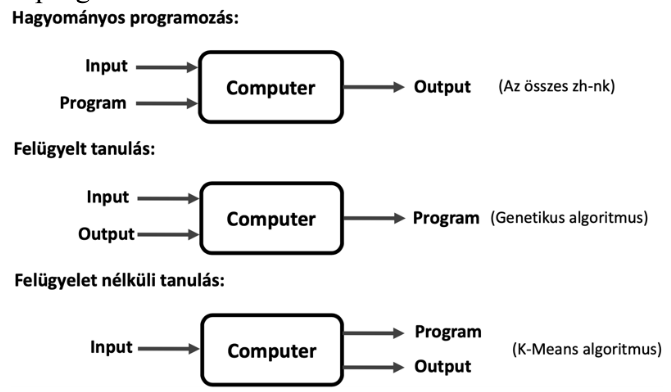
\includegraphics[width=0.6\textwidth]{res/imgs/info_25_learning_types.png}
    \end{center}
\end{itemize}

\textbf{Perceptron:}
\begin{itemize}
    \item egyrétegű perceptron
    \begin{itemize}
        \item legegyszerűbb formájú neurális hálózat
        \item minták osztályozására használják fel
        \item McCulloch-Pitts féle neuron modellen alapul
    \end{itemize}
    \item mesterséges neuron:
    \begin{center}
        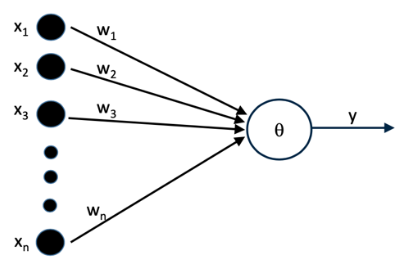
\includegraphics[width=0.4\textwidth]{res/imgs/info_25_artificial_neuron.png}
    \end{center}
    \begin{itemize}
        \item bemenetek: bejövő jelek $x_i$
        \item kimenet: klaszifikáció $y$
        \item súlyok: $w_i$
        \item küszöb: $\Theta$
        \item csak néhány egyszerű információ feldolgozására képes
        \item nem képes összetett problémák megoldására
        \item neuronok összekötve képesek komplex viselkedésre, így használhatók komplex problémák megoldására
    \end{itemize}
    \item egyrétegű perceptron
    \begin{center}
        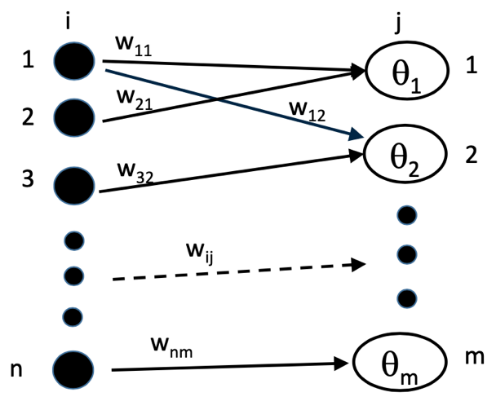
\includegraphics[width=0.4\textwidth]{res/imgs/info_25_single_layer_perceptron.png}
    \end{center}
    \begin{equation*}
        out_j = sgn\left( \sum_{i=1}^n out_i w_{ij} - \theta_j \right)
    \end{equation*}
    \begin{itemize}
        \item tetszőleges számú McCulloch-Pitts féle neuront összerendezhetünk
        \item egy lehetséges elrendezés: egy rétegben helyezzük el a mesterséges neuronokat
        \item ez a perceptron
        \item csak lineárisan szeparálható minták osztályozására használjuk
        \item nemlineáris minták osztályozására nem jó
        \item a többrétegű perceptronok képesek lineárisan nem szeparálható minták osztályozására
    \end{itemize}
    \begin{center}
        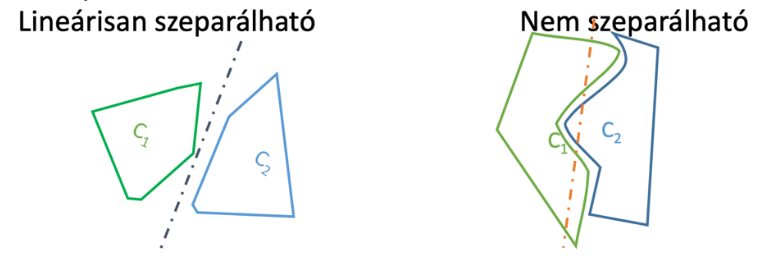
\includegraphics[width=0.6\textwidth]{res/imgs/info_25_separability.png}
    \end{center}
    \item logikai kapuk megvalósítása:
    \begin{itemize}
        \item súlyokat és küszöbértékeket kell megállapítani
        \item NOT, OR, AND kapukat tudunk megvalósítani, XOR-t nem
        \item ezekkel minden logikai hálózat megvalósítható
        \item felügyelt tanulás, ismert bemenetek és kimenet
        \item minden tanító minta egy lineáris egyenlőtlenséget ír le a kimenet számára. a bemenetek és a hálózat paraméterei alapján -> ezeket használjuk a súlyok és a küszöbérték meghatározására
    \end{itemize}
    \begin{center}
        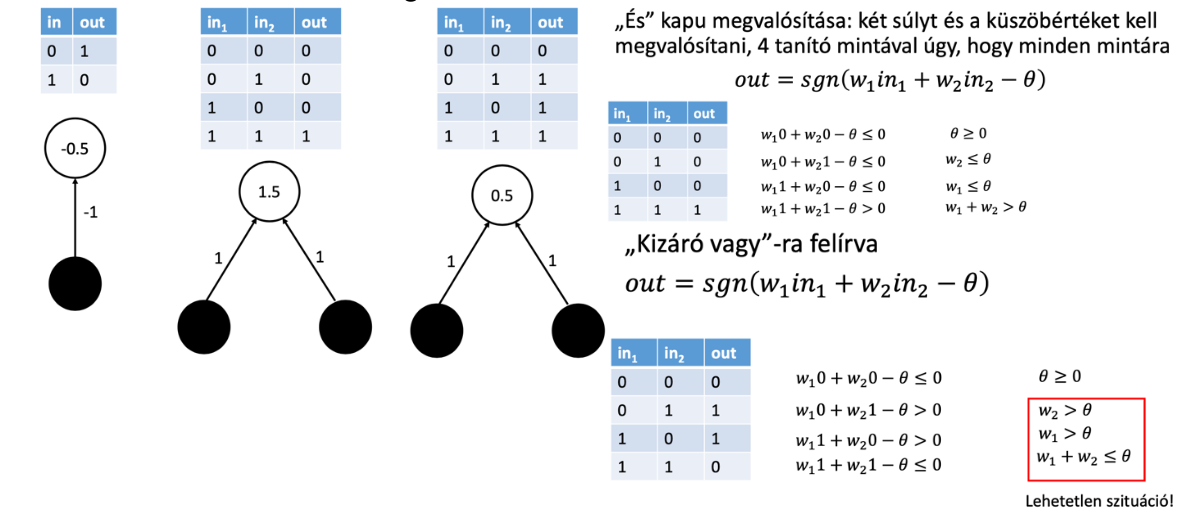
\includegraphics[width=0.95\textwidth]{res/imgs/info_25_logic_gates.png}
    \end{center}
    \item perceptron tanítása:
    \begin{itemize}
        \item tanítási algoritmus
        \item a tanító minták, és az elvárt kimenet ($d$) adottak
        \item 1. kezdeti inicializálás:
        \begin{center}
            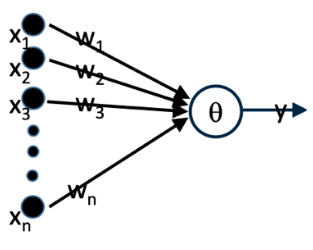
\includegraphics[width=0.3\textwidth]{res/imgs/info_25_training_initialization.png}
        \end{center}
        \begin{itemize}
            \item állítsunk be kezdeti értékeket a súlyoknak
            \item állítsunk be a küszöbértéknek egy -0,5 és 0,5 közötti számot
            \item állítsuk be a $\eta$ tanulási paramétert 1-nél kisebb pozitív értékre
        \end{itemize}
        \item 2. aktiválás:
        \begin{center}
            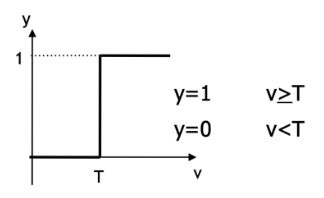
\includegraphics[width=0.3\textwidth]{res/imgs/info_25_activation_function.png}
        \end{center}
        \begin{itemize}
            \item számítsuk ki a tényleges a p=1 iterációs lépésben, a kimenetre lépés aktivációs függvényt alkalmazva
        \end{itemize}
        \item 3. súlyok tanulása:
        \begin{itemize}
            \item számítsuk ki a tényleges kimenet és az elvárt kimenet közti hibát a p-edik lépésben: $e(p) = d(p) - y(p)$
            \item korrigáljuk a súlyokat: $\Delta w_i(p) = \eta \cdot x_i(p) \cdot e(p)$
            \item új súly: $w_i(p+1) = w_i(p) + \Delta w_i(p)$
        \end{itemize}
        \item 4. iteráció: növeljük $p$ értékét eggyel, menjünk vissza a 2-es lépésre, ismételjük addig, amíg nincs konvergencia
    \end{itemize}
\end{itemize}